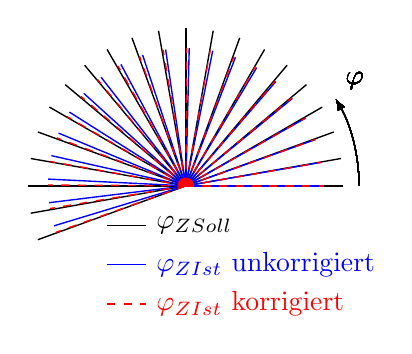
\begin{tikzpicture}
%
%Wunsch
%
\foreach \x in
{0,10,20,30,40,50,60,70,80,90,100,110,120,130,140,150,160,170,180,190,200}
%
\draw[line width =0.5pt](0,0)--(\x:2);
%
%Ohne Korrektur
%
\foreach \x in
{0,9.84375,19.6875,29.53125,39.375,49.21875,59.0625,68.90625,78.75,88.59375,98.4375,108.28125,118.125,127.96875,137.8125,147.65625,157.5,167.34375,177.1875,187.03125,196.875}
%
\draw[blue,line width =0.5pt](0,0)--(\x:1.75);
%
%Mit Korrektur
%
\foreach \x in
{0,9.84375,19.6875,29.53125,39.726562,49.570312,59.765625,69.609375,
79.804688,89.648438,99.492188,109.6875,119.53125,129.72656,139.57031,
149.76562,159.60938,169.80469,179.64844,189.49219,199.6875}
%
\visible<2->{\draw[red,line width =0.5pt,dashed](0,0)--(\x:1.75);}
%
\draw[-latex] (0:2.2) arc (0:30:2.2)node[above right]{$\varphi$};
%
%Legende
%
\draw[line width =0.5pt]
(-1,-0.5)--(-0.5,-0.5)node[right]{$\varphi_{Z\text{Soll}}$}; 
\draw[blue,line width =0.5pt]
(-1,-1)--(-0.5,-1)node[right]{$\varphi_{Z\text{Ist}}$ unkorrigiert}; 
%
\visible<2->{\draw[red,line width
=0.5pt,dashed] (-1,-1.5)--(-0.5,-1.5)node[right]{$\varphi_{Z\text{Ist}}$
korrigiert};}
%
\end{tikzpicture}